\documentclass[12pt]{beamer}
\usepackage{../Estilos/BeamerFC}
\usepackage{../Estilos/ColoresLatex}
\usepackage{courier}
\usepackage{listingsutf8}
\usepackage{listings}
\usepackage{xcolor}
\usepackage{textcomp}
\usepackage{color}
\definecolor{deepblue}{rgb}{0,0,0.5}
\definecolor{brown}{rgb}{0.59, 0.29, 0.0}
\definecolor{OliveGreen}{rgb}{0,0.25,0}
% \usepackage{minted}

\DeclareCaptionFont{white}{\color{white}}
\DeclareCaptionFormat{listing}{\colorbox{gray}{\parbox{0.98\textwidth}{#1#2#3}}}
\captionsetup[lstlisting]{format=listing,labelfont=white,textfont=white}
\renewcommand{\lstlistingname}{Código}


\definecolor{Code}{rgb}{0,0,0}
\definecolor{Keywords}{rgb}{255,0,0}
\definecolor{Strings}{rgb}{255,0,255}
\definecolor{Comments}{rgb}{0,0,255}
\definecolor{Numbers}{rgb}{255,128,0}

\makeatletter

\newif\iffirstchar\firstchartrue
\newif\ifstartedbyadigit
\newif\ifprecededbyequalsign

\newcommand\processletter
{%
  \ifnum\lst@mode=\lst@Pmode%
    \iffirstchar%
        \global\startedbyadigitfalse%
      \fi
      \global\firstcharfalse%
    \fi
}

\newcommand\processdigit
{%
  \ifnum\lst@mode=\lst@Pmode%
      \iffirstchar%
        \global\startedbyadigittrue%
      \fi
      \global\firstcharfalse%
  \fi
}

\lst@AddToHook{OutputOther}%
{%
  \lst@IfLastOtherOneOf{=}
    {\global\precededbyequalsigntrue}
    {}%
}

\lst@AddToHook{Output}%
{%
  \ifprecededbyequalsign%
      \ifstartedbyadigit%
        \def\lst@thestyle{\color{orange}}%
      \fi
    \fi
  \global\firstchartrue%
  \global\startedbyadigitfalse%
  \global\precededbyequalsignfalse%
}

\lstset{ 
language=Python,                % choose the language of the code
basicstyle=\footnotesize\ttfamily,       % the size of the fonts that are used for the code
numbers=left,                   % where to put the line-numbers
numberstyle=\scriptsize,      % the size of the fonts that are used for the line-numbers
stepnumber=1,                   % the step between two line-numbers. If it is 1 each line will be numbered
numbersep=5pt,                  % how far the line-numbers are from the code
backgroundcolor=\color{white},  % choose the background color. You must add \usepackage{color}
showspaces=false,               % show spaces adding particular underscores
showstringspaces=false,         % underline spaces within strings
showtabs=false,                 % show tabs within strings adding particular underscores
frame=single,   		% adds a frame around the code
tabsize=2,  		% sets default tabsize to 2 spaces
captionpos=t,   		% sets the caption-position to bottom
breaklines=true,    	% sets automatic line breaking
breakatwhitespace=false,    % sets if automatic breaks should only happen at whitespace
escapeinside={| |},  % if you want to add a comment within your code
stringstyle =\color{OliveGreen},
otherkeywords={as, np.array, np.concatenate, np.linspace, linspace, interpolate.interp1d, kind, plt.plot, .copy, np.arange, np.cos, np.pi, lw, ls, label, splrep, splev, plt.legend, loc, plt.title, plt.ylim, plt.show, sign, math.ceil, math.log, np.sqrt, np.exp, np.zeros, plt.xlabel, plt.ylabel, plt.xlim, np.identity, random, np.dot, np.outer, np.diagonal },             % Add keywords here
keywordstyle = \color{blue},
commentstyle = \color{darkcerulean},
identifierstyle = \color{black},
literate=%
         {á}{{\'a}}1
         {é}{{\'e}}1
         {í}{{\'i}}1
         {ó}{{\'o}}1
         {ú}{{\'u}}1
%
%keywordstyle=\ttb\color{deepblue}
%fancyvrb = true,
}

\lstdefinestyle{FormattedNumber}{%
    literate={0}{{\textcolor{red}{0}}}{1}%
             {1}{{\textcolor{red}{1}}}{1}%
             {2}{{\textcolor{red}{2}}}{1}%
             {3}{{\textcolor{red}{3}}}{1}%
             {4}{{\textcolor{red}{4}}}{1}%
             {5}{{\textcolor{red}{5}}}{1}%
             {6}{{\textcolor{red}{6}}}{1}%
             {7}{{\textcolor{red}{7}}}{1}%
             {8}{{\textcolor{red}{8}}}{1}%
             {9}{{\textcolor{red}{9}}}{1}%
             {.0}{{\textcolor{red}{.0}}}{2}% Following is to ensure that only periods
             {.1}{{\textcolor{red}{.1}}}{2}% followed by a digit are changed.
             {.2}{{\textcolor{red}{.2}}}{2}%
             {.3}{{\textcolor{red}{.3}}}{2}%
             {.4}{{\textcolor{red}{.4}}}{2}%
             {.5}{{\textcolor{red}{.5}}}{2}%
             {.6}{{\textcolor{red}{.6}}}{2}%
             {.7}{{\textcolor{red}{.7}}}{2}%
             {.8}{{\textcolor{red}{.8}}}{2}%
             {.9}{{\textcolor{red}{.9}}}{2}%
             {\ }{{ }}{1}% handle the space
         ,%
          %mathescape=true
          escapeinside={__}
          }



\usetheme{Warsaw}
\usecolortheme{seahorse}
%\useoutertheme{default}
\setbeamercovered{invisible}
% or whatever (possibly just delete it)
\setbeamertemplate{section in toc}[sections numbered]
\setbeamertemplate{subsection in toc}[subsections numbered]
\setbeamertemplate{subsection in toc}{\leavevmode\leftskip=3.2em\rlap{\hskip-2em\inserttocsectionnumber.\inserttocsubsectionnumber}\inserttocsubsection\par}
\setbeamercolor{section in toc}{fg=blue}
\setbeamercolor{subsection in toc}{fg=blue}
\setbeamercolor{frametitle}{fg=blue}
\setbeamertemplate{caption}[numbered]

\setbeamertemplate{footline}
\beamertemplatenavigationsymbolsempty
\setbeamertemplate{headline}{}


\makeatletter
\setbeamercolor{section in foot}{bg=gray!30, fg=black!90!orange}
\setbeamercolor{subsection in foot}{bg=blue!30}
\setbeamercolor{date in foot}{bg=black}
\setbeamertemplate{footline}
{
  \leavevmode%
  \hbox{%
  \begin{beamercolorbox}[wd=.333333\paperwidth,ht=2.25ex,dp=1ex,center]{section in foot}%
    \usebeamerfont{section in foot} \insertsection
  \end{beamercolorbox}%
  \begin{beamercolorbox}[wd=.333333\paperwidth,ht=2.25ex,dp=1ex,center]{subsection in foot}%
    \usebeamerfont{subsection in foot}  \insertsubsection
  \end{beamercolorbox}%
  \begin{beamercolorbox}[wd=.333333\paperwidth,ht=2.25ex,dp=1ex,right]{date in head/foot}%
    \usebeamerfont{date in head/foot} \insertshortdate{} \hspace*{2em}
    \insertframenumber{} / \inserttotalframenumber \hspace*{2ex} 
  \end{beamercolorbox}}%
  \vskip0pt%
}
\makeatother

\makeatletter
\patchcmd{\beamer@sectionintoc}{\vskip1.5em}{\vskip0.8em}{}{}
\makeatother

%\newlength{\depthofsumsign}
%\setlength{\depthofsumsign}{\depthof{$\sum$}}
% \newcommand{\nsum}[1][1.4]{% only for \displaystyle
%     \mathop{%
%         \raisebox
%             {-#1\depthofsumsign+1\depthofsumsign}
%             {\scalebox
%                 {#1}
%                 {$\displaystyle\sum$}%
%             }
%     }
% }
\def\scaleint#1{\vcenter{\hbox{\scaleto[3ex]{\displaystyle\int}{#1}}}}
\def\scaleoint#1{\vcenter{\hbox{\scaleto[3ex]{\displaystyle\oint}{#1}}}}
\def\bs{\mkern-12mu}

\usefonttheme{serif}

\title{Tema 0 - Introducción a python 3}
\author{M. en C. Gustavo Contreras Mayén}
\date{21 de agosto de 2023}

\begin{document}

\maketitle

\section*{Contenido}
\frame[allowframebreaks]{\frametitle{Contenido}\tableofcontents[currentsection, hideallsubsections]}

\section{Funciones}
\frame[allowframebreaks]{\frametitle{Contenido}\tableofcontents[currentsection, hideothersubsections]}
\subsection{¿Para qué usar funciones?}

\begin{frame}
\frametitle{¿Qué es una función?}
Una función es un fragmento aislado de código, que tiene un \emph{nombre}, con un parámetro, o más parámetros o ninguno y devuelve un valor.
\end{frame}
\begin{frame}
\frametitle{¿Para qué usar una función?}
En general, una función hará algo por nosotros ocupando para ello los parámetros de entrada que le indiquemos, normalmente devolverá un resultado.
\\
\bigskip
\pause
No estamos limitados a usar las \emph{funciones intrínsecas} en la biblioteca estándar o las proporcionadas por terceros. \pause ¡También podemos escribir nuestras propias funciones!
\end{frame}
\begin{frame}   
\frametitle{Ventajas al usar funciones}
Hay buenas razones por las que las funciones son un componente clave en la programación:
\setbeamercolor{item projected}{bg=flame,fg=flavescent}
\setbeamertemplate{enumerate items}{%
\usebeamercolor[bg]{item projected}%
\raisebox{1.5pt}{\colorbox{bg}{\color{fg}\footnotesize\insertenumlabel}}%
}
\begin{enumerate}[<+->]
\item Encapsulación: envolver una parte de código útil en una función para que pueda usarse sin conocimiento de los detalles.
\item Generalización: hacer que una parte de código sea útil en diversas circunstancias a través de parámetros.
\item Manejo: Dividir un programa complejo en partes fáciles de manejar.
\seti
\end{enumerate}
\end{frame}
\begin{frame}
\frametitle{Ventajas al usar funciones}
\setbeamercolor{item projected}{bg=flame,fg=flavescent}
\setbeamertemplate{enumerate items}{%
\usebeamercolor[bg]{item projected}%
\raisebox{1.5pt}{\colorbox{bg}{\color{fg}\footnotesize\insertenumlabel}}%
}
\begin{enumerate}[<+->]
\conti
\item Mantenimiento: uso de nombres significativos para hacer que el programa sea más legible y comprensible.
\item Reutilización: una buena función puede ser útil en múltiples programas.
\item Recursión!
\end{enumerate}
\end{frame}

\subsection{Funciones incluidas}

\begin{frame}[fragile]
\frametitle{Funciones incluidas en \python}
Sin requerir la llamada a un módulo o librería, hay funciones de \python{} que se pueden ocupar en todo momento.
\\
\bigskip
\pause
Más adelante veremos que en \python{} se incluyen librerías matemáticas que nos serán de utilidad, por lo que ocuparlas también requiere de un uso particular.
\end{frame}
\begin{frame}
\frametitle{Usando funciones disponibles}
En el siguiente ejemplo se revisan algunas funciones disponibles en \python, \pause para conocer más sobre las mismas, recuerda que puedes ocupar la documentación oficial.
\end{frame}
\begin{frame}[fragile]
\frametitle{Funciones incluidas en \python}
\begin{lstlisting}[caption=Funciones incluidas]
print(abs(-3))
print()
print(bin(8))
print()
print(len('Pumas'))
print()
print(max([1, 3.1416, 100, 1E2]))
print()
print(pow(5,2))
\end{lstlisting}
\end{frame}

\subsection{Funciones definidas por el usuario}

\begin{frame}
\frametitle{Funciones creadas por el usuario}
Para facilitarnos la solución de problemas, será neceario crear nuestras propias funciones, por lo que hay que seguir una serie de reglas importantes para ello.
\end{frame}
\begin{frame}[fragile]
\frametitle{Estructura de una función}
La palabra reservada \funcionazul{def} se usa para definir funciones. 
\\
\bigskip
\pause
Debe seguirle el nombre de la función y la lista de parámetros formales entre paréntesis. Las sentencias que forman el cuerpo de la función empiezan en la línea siguiente, y deben estar con sangría.
\end{frame}
\begin{frame}[fragile]
\frametitle{Estructura de una función}
La estructura de una función en \python{} es la siguiente:
\begin{center}
\fontsize{12}{12}\selectfont
\begin{exampleblock}{}
\verb| def nombre_funcion(parametro1, ...):|
\verb|     conjunto de instrucciones|
\verb|     return valores_devueltos|
\end{exampleblock}
\end{center}
Un parámetro puede ser cualquier objeto de \python, incluyendo una función. \pause Los parámetros pueden darse por defecto, por lo que en la función son opcionales. 
\end{frame}
\begin{frame}
\frametitle{Lo que devuelve una función}
Una función no necesariamente devuelve algún valor, ya que por ejemplo, se puede crear una función para dar formato a una cadena.
\\
\bigskip
\pause
Si queremos devolver un valor al código principal, se utiliza la instrucción \funcionazul{return}.
\end{frame}
\begin{frame}[fragile]
\frametitle{Ejemplo}
\begin{lstlisting}[caption=Función sencilla,basicstyle=\linespread{1.2}\ttfamily\small, columns=fullflexible,escapeinside=||]
def cuadrados(a):
	for i in range(len(a)):
		a[i] = a[i]**2
    return a

a = [1, 2, 3, 4]

solucion = cuadrados(a)

print(solucion)
\end{lstlisting}
\end{frame}
\begin{frame}
\frametitle{Cálculo de la serie de Fibonacci}
La sucesión fue descrita por Fibonacci como la solución a un problema de la cría de conejos: 
\\
\bigskip
\enquote{Cierto hombre tenía una pareja de conejos juntos en un lugar cerrado y uno desea saber cuántos son creados a partir de este par en un año, .cuando es su naturaleza parir otro par en un simple mes, y en el segundo mes los nacidos parir también}
\\
\bigskip
\pause
\textcolor{red}{¿Cómo le hacemos?}
\end{frame}
\begin{frame}[fragile]
\frametitle{Propuesta de código}
\begin{lstlisting}[caption=Primer intento para la serie de Fibonacci, basicstyle=\linespread{1.2}\ttfamily\small, columns=fullflexible,escapeinside=||]
def fib(n):
    a, b = 0, 1
    while b < n:
        print (b)
        a, b = b, a + b
    return b

f = fib(2000)
print(f)
\end{lstlisting}
\pause
\end{frame}

\subsection{Paso de argumentos}

\begin{frame}[fragile]
\frametitle{Paso de argumentos}
Para que una función sea en verdad útil (y reutilizable), es necesario que podamos pasarle entradas. 
\\
\bigskip
Los nombres de las entradas (o argumentos) que requiere una función se declaran a continuación del nombre en \funcionazul{def} (siempre entre paréntesis)
\end{frame}
\begin{frame}[fragile]
\frametitle{Paso de argumentos}
\begin{lstlisting}[caption=Paso de argumentos en una función, basicstyle=\linespread{1.2}\ttfamily\small, columns=fullflexible,escapeinside=||]
def funcion_suma(x, y):
    return x + y

print(funcion_suma(5, 3))
print()
print(funcion_suma(7, 42.0))
print()
print(funcion_suma("Hola ", " Mundo!"))
\end{lstlisting}
\end{frame}
\begin{frame}[fragile]
\frametitle{Paso de argumentos}
\textbf{Nota:} 
\begin{itemize}[<+->]
\item[\ding{212}] Nunca se mencionan los tipos de datos de $x$ e $y$, ni el tipo de datos que devuelve \funcionazul{funcion\_suma}.
\item[\ding{212}] Los argumentos y el valor devuelto son, tal como las variables, simples etiquetas a zonas de memoria.
\end{itemize}  
\end{frame}

\subsection{Paso de argumento con nombre}

\begin{frame}
\frametitle{Paso de argumentos con nombre}
Si la función que definimos tiene muchos argumentos, es fácil olvidar el orden en que fueron declarados.
\\
\bigskip
\pause
Como un argumento no lleva asociado un tipo, \python{} no tiene manera de saber que los argumentos están cambiados.
\end{frame}
\begin{frame}
\frametitle{Paso de argumentos con nombre}
Para evitar este tipo de errores, hay una manera de llamar a una función pasando los argumentos en cualquier orden arbitrario: \textcolor{blue}{los argumentos se pasan usando el nombre usado en la declaración}.
\end{frame}
\begin{frame}[fragile]
\frametitle{Ejemplo de paso de argumentos con nombre}
\begin{lstlisting}[caption=Paso de argumentos con nombre,basicstyle=\linespread{1.2}\ttfamily\small, columns=fullflexible,escapeinside=||]
def prueba(a, b, c):
    print("a = {0:}, b = {1:}, c = {2:}".format(a, b, c))

prueba(1, 2, 3)
print()
prueba(b=3, a=2, c=1)
\end{lstlisting}
\end{frame}

\subsection{Argumentos con valores por omisión}

\begin{frame}[fragile]
\frametitle{Argumentos con valores por omisión}
Para hacer que algunos argumentos sean opcionales, se les asignan valores por omisión al declararlos.
\\
\bigskip
\pause
En el siguiente ejemplo se muestra el caso cuando se define la función con dos argumentos y se indica solo uno.
\end{frame}
\begin{frame}[fragile]
\frametitle{Argumentos con valores por omisión}    
\begin{lstlisting}[caption=Ejemplo cuando se omiten argumentos declarados, basicstyle=\linespread{1.2}\ttfamily\small, columns=fullflexible,escapeinside=||]
from math import sqrt

# argumento v es requerido , c es opcional
# c toma el valor 3.0e8 por omision

def tau_cero(v, c = 3.0e+8):
    return sqrt(1.0 - (v/c)**2)

print(tau_cero(0.1 , 1.0))
print()
print(tau_cero(1.e+7)) # usa c = 3.0e+8
\end{lstlisting}
\end{frame}

\subsection{Regresando varios valores}

\begin{frame}[fragile]
\frametitle{Regresando varios valores en una función}
Para hacer que una función devuelva más de un valor, en lenguajes como Fortran, C o C++, lo que se hace es definir argumentos de entrada y argumentos de salida.
\end{frame}
\begin{frame}[fragile]
\frametitle{Regresando varios valores en una función}
Para devolver múltiples valores en \python, lo usual es devolver los valores \enquote{empaquetados} en una tupla.
\\
\bigskip
\pause
En el siguiente ejemplo se revisa este caso, checa la referencia para presentar el formato de la cadena y valor numérico de la variable argumento.
\end{frame}
\begin{frame}[fragile]
\frametitle{Regresando varios valores en una función}
\begin{lstlisting}[caption=Devolviendo varios valores, basicstyle=\linespread{1.2}\ttfamily\small, columns=fullflexible,escapeinside=||]
from math import atan2, sqrt

def modulo_argumento(x, y):
    norm = sqrt(x**2 + y**2)
    arg = atan2(y, x)
    return (norm, arg)
    
n, a = modulo_argumento(3.0, 4.0)
print("El modulo es: {0:}".format(n))
print("El argumento es: {0:.4f}".format(a))
\end{lstlisting}
\end{frame}

\subsection{Número variable de argumentos}

\begin{frame}[fragile]
\frametitle{Número variable de argumentos}
Hasta el momento hemos revisado que una función con un número determinado de parámetros, debe de llamarse con ese número de parámetros.
\\
\bigskip
\pause
Si nos hace falta alguno, o escribimos un argumento demás, nos marcará un error.
\end{frame}
\begin{frame}[fragile]
\frametitle{Número variable de argumentos}    
¿Cómo le hacemos para que una función acepte un número no prefijado de argumentos?
\\
\
\pause
Es posible pasar una lista o tupla, pero \python\ ofrece una mejor solución:
\end{frame}
\begin{frame}[fragile]
\frametitle{Número variable de argumentos}
\begin{lstlisting}[caption=Uso de *args, basicstyle=\linespread{1.2}\ttfamily\footnotesize, columns=fullflexible,escapeinside=||]
import math

def miatan(*args):
# args es una tupla de argumentos
    if len(args) == 1:
        return math.atan(args[0])
    else :
        return math.atan2(args[0],args[1])

print(miatan (0.2)) # 0.19739
print(miatan (2.0, 10.0)) # 0.19739
print(miatan (-2.0, -10.0)) # -2.94419
\end{lstlisting}
\end{frame}

\subsection{Funciones lambda}

\begin{frame}
\frametitle{Funciones lambda}
\python\ admite una interesante sintaxis que permite definir funciones mínimas, de una línea, sobre la marcha. 
\\
\bigskip
\pause
Se trata de las denominadas funciones \azulfuerte{lambda}, que pueden utilizarse en cualquier lugar donde se necesite una función.
\end{frame}
\begin{frame}[allowframebreaks, fragile]
\frametitle{Funciones lambda}
\begin{lstlisting}[caption=Ejemplo de función lambda,basicstyle=\linespread{1.2}\ttfamily\small, columns=fullflexible,escapeinside=||]
cuadrado = lambda x: x**2
print(cuadrado(3))
#Devuelve 9

print((lambda x: x**2)(3))
#se usa lambda dentro del print
\end{lstlisting}
\end{frame}
\begin{frame}
\frametitle{Funciones lambda}
Nótese que:
\setbeamercolor{item projected}{bg=bistre,fg=beige}
\setbeamertemplate{enumerate items}{%
\usebeamercolor[bg]{item projected}%
\raisebox{1.5pt}{\colorbox{bg}{\color{fg}\footnotesize\insertenumlabel}}%
}
\begin{enumerate}[<+->]
\item La lista de argumentos no está entre paréntesis.
\item Falta la palabra reservada \azulfuerte{return} (está implícita, ya que la función entera debe ser una única expresión). 
\item La función no tiene nombre, pero puede ser llamada mediante la variable a que se ha asignado.
\end{enumerate}
\end{frame}

\section{Módulos}
\frame[allowframebreaks]{\tableofcontents[currentsection, hideothersubsections]}
\subsection{Módulos en \python}

\begin{frame}[fragile]
\frametitle{Módulos}
Es una buena práctica de programación que almacenemos las funciones en módulos.
\\
\bigskip
\pause
Un módulo es un archivo de \python{} en donde se dejan las funciones que hemos construido, el nombre del módulo es el nombre del archivo.
\end{frame}
\begin{frame}
\frametitle{Ventaja de usar módulos}
Cuando creamos un módulo, todas las funciones están disponibles para cualquiera de los programas que estemos generando.
\\
\bigskip
\pause
Basta con identificar la ruta del archivo y hacer la referencia dentro de nuestro programa.
\end{frame}
\begin{frame}[fragile]
\frametitle{Uso de los módulos}
Un módulo se carga al programa con la instrucción:
\pause
\funcionazul{
\begin{center}
\texttt{from nombre\_modulo import *}
\end{center}
}
\python\ incluye un número grande de módulos que contienen funciones y métodos para varias tareas. 
\end{frame}
\begin{frame}[fragile]
\frametitle{Usando el módulo \texttt{math}}
Muchas funciones matemáticas no se pueden llamar directo del intérprete, \pause anteriormente se revisaron algunas de las funciones incluidas, \pause para ocupar un conjunto de funciones matemáticas, ocupamos el módulo \funcionazul{math}.
\end{frame}
\begin{frame}[fragile]
\frametitle{Usando el módulo \texttt{math}}
Hay tres diferentes maneras en las que se puede llamar y utilizar las funciones de un módulo.
\begin{exampleblock}{}
\verb|from math import *|
\end{exampleblock}
\end{frame}
\begin{frame}
\frametitle{Usando el módulo \texttt{math}}
De esta manera, se importan todas las funciones definidas en el módulo \funcionazul{math}, siendo quizá un gasto innecesario de recursos, pero también generar conflictos con definiciones cargadas de otros módulos.
\end{frame}
\begin{frame}[fragile]
\frametitle{Segunda forma de llamar a \texttt{math}}
\begin{exampleblock}{}
\verb|from math import func1, func2,...|
\end{exampleblock}
\pause
\begin{exampleblock}{}
\verb|>>> from math import log, sin| \\
\verb|>>> print (log(sin(0.5)))| \\
\verb|-0.735166686385|
\end{exampleblock}
\end{frame}
\begin{frame}[fragile]
\frametitle{Usando el módulo \texttt{math}}
El tercer método es el más usado en programación, dejando disponible el módulo:
\begin{center}
\verb|import math|
\end{center}
\pause
Las funciones en el módulo se pueden usar con el nombre del módulo como prefijo:
\pause
\begin{exampleblock}{}
\verb|>>> import math| \\
\verb|>>> print (math.log(math.sin(0.5)))|
\verb|-0.735166686385|
\end{exampleblock}
\end{frame}
\begin{frame}
\frametitle{Consideraciones}
Hay que tomar en cuenta que: habrá funciones que existen dentro del módulo \texttt{math}, \pause pero también con el mismo nombre las encontraremos en otros módulos: \funcionazul{numpy} y \funcionazul{scipy}.
\\
\bigskip
\pause
Por ello se recomienda el uso de \enquote{alias} que nos permitan identificar el módulo origen de la función.
\end{frame}
\begin{frame}[fragile]
\frametitle{Contenido del módulo \texttt{math}}
Podemos ver el contenido de un módulo con la instrucción:
\\
\verb|>>> import math| \\
\verb|>>> dir(math)|
\fontsize{10}{10}\selectfont
\begin{verbatim}
['__doc__', '__name__', '__package__', 'acos',
'acosh',  'asin', 'asinh', 'atan', 'atan2',
'atanh', 'ceil', 'copysign', 'cos', 'cosh',
'degrees', 'e', 'erf', 'erfc', 'exp', 'expm1',
'fabs', 'factorial', 'floor', 'fmod', 'frexp',
'fsum', 'gamma', 'hypot', 'isinf', 'isnan',
'ldexp', 'lgamma', 'log', 'log10', 'log1p',
'modf', 'pi', 'pow', 'radians', 'sin', 'sinh',
'sqrt', 'tan', 'tanh', 'trunc']
\end{verbatim}
\end{frame}

\section{Graficación con python}
\frame{\tableofcontents[currentsection, hideothersubsections]}
\subsection{Librería matplotlib}

\begin{frame}
\frametitle{Graficación con \python}
Una buena parte del trabajo que tendremos que hacer como físicos es utilizar un conjunto de datos que por si solos, no van a darnos información sobre un modelo o un fenómeno, por ello, será necesario usar gráficas.
\\
\medskip
\pause
En \python{} se incluye un módulo de graficación bastante versátil para generar gráficas y exportarlas a diferentes tipos de archivos. \pause La librería se llama \funcionazul{matplotlib}.
\end{frame}
\begin{frame}
\frametitle{La librería \texttt{matplotlib.pyplot}}
Es una colección de funciones de estilo de mando, de tal manera que \funcionazul{matplotlib} funciona a la manera de \texttt{MATLAB}.
\\
\bigskip
\pause
Cada instrucción \funcionazul{pyplot} aplica un cambio a una figura: por ejemplo, crear una figura, crear un área de trazado en una figura, dibujar algunas líneas en un área de trazado, decorar con etiquetas, etc.
\end{frame}
\begin{frame}[fragile]
\frametitle{Ejercicio 1}
\begin{lstlisting}[caption=Primer ejercicio de graficación]
import matplotlib.pyplot as plt

plt.plot([1, 2, 3, 4])
plt.ylabel('Algunos numeros')
plt.show()
\end{lstlisting}
\end{frame}
\begin{frame}[fragile]
\frametitle{Ejercicio de graficación 1}
\begin{figure}
	\centering
	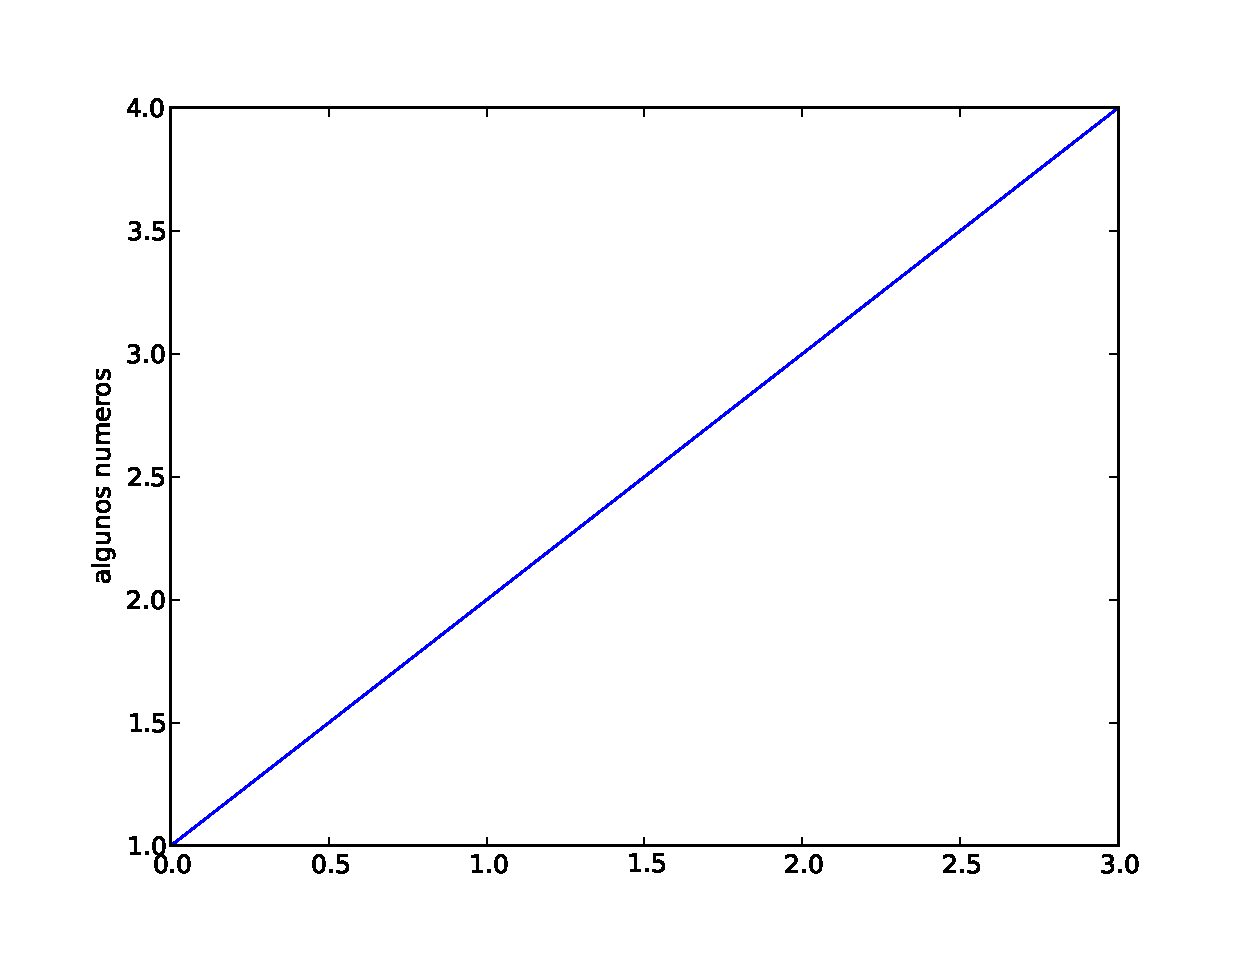
\includegraphics[scale=0.35]{Imagenes/plotEjercicio1.eps}<2> 
\end{figure}
\end{frame}
\begin{frame}
\frametitle{Entendiendo la gráfica obtenida}
Te estarás preguntando: ¿por qué tenemos en el eje $x$ el rango $0-3$ y en el eje $y$ el rango  $1-4$?.
\\
\medskip
\pause
Si proporcionamos una única lista o matriz en el comando \funcionazul{plot}, \funcionazul{matplotlib} asume que es una secuencia de valores de $y$, \pause por lo que genera automáticamente los valores de $x$ para nosotros.
\end{frame}
\begin{frame}
\frametitle{Entendiendo la gráfica obtenida}
Como los índices en \python{} comienzan en $0$, el vector $x$ por defecto tiene la misma longitud que $y$, pero inicia con $0$.
\\
\bigskip
\pause
De ahí que los datos en el eje $x$ son: $[0, 1, 2, 3]$.
\end{frame}
\begin{frame}[fragile]
\frametitle{Ejercicio de graficación 2}
\begin{lstlisting}[caption=Graficando dos listas]
import matplotlib.pyplot as plt

plt.plot([1, 2, 3, 4], [1, 4, 9, 16], 'ro')
plt.axis([0, 6, 0, 20])
plt.show()
\end{lstlisting}
\end{frame}
\begin{frame}[fragile]
\frametitle{Ejercicio de graficación 2}
\begin{figure}
	\centering
	\includegraphics[scale=0.475]{Imagenes/plotEjercicio2.eps}<2> 
\end{figure}
\end{frame}
\begin{frame}
\frametitle{Consideración importante}
Nótese que se grafican solo los puntos, \pause no hay una línea que los conecte.
\\
\bigskip
\pause
La unión de los puntos a veces ayuda para entender la visualización, pero no debemos de asumir que el comportamiento de los datos siempre debe de ser una línea que una los puntos.
\end{frame}
\begin{frame}[fragile]
\frametitle{Interpretando la gráfica}
Por cada par $x$, $y$ de argumentos, existe un tercer argumento opcional: que es la cadena de formato que indica el \emph{color} y el \emph{tipo de línea}, en el ejemplo \texttt{'ro' = red o} (círculo).
\\
\medskip
\pause
Las letras y los símbolos de la cadena de formato se concatenanen una cadena de color y estilo de línea. \pause La cadena de formato por defecto es \verb|'b-'|, que es una línea de color azul.
\end{frame}
\begin{frame}[fragile]
\frametitle{Tipos de líneas}
\renewcommand{\arraystretch}{0.9}
\begin{tabular}{l | l}
carácter & descripción \\ \hline
\verb|'-'|	& línea sólida \\ \hline
\verb|'--'| & línea cortada \\ \hline
\verb|'-.'| & línea-punto \\ \hline
\verb|':'|	& línea de puntos \\ \hline
\verb|'.'|	& marca de punto \\ \hline
\verb|','|	& marca de pixel \\ \hline
\verb|'o'|	& marca de círculo \\ \hline
\verb|'v'|	& marca de triándulo hacia abajo \\ \hline
\verb|'^'|	& marca de triángulo hacia arriba
\end{tabular}
\end{frame}
\begin{frame}[fragile]
\frametitle{Lista de colores}
\renewcommand{\arraystretch}{0.8}
\begin{tabular}{l | l}
carácter & color \\ \hline
\verb|'b'| & azul \\ \hline
\verb|'g'| & verde \\ \hline
\verb|'r'| & rojo \\ \hline
\verb|'c'| & cyan \\ \hline
\verb|'m'| & magenta \\ \hline
\verb|'y'| & amarillo \\ \hline
\verb|'k'| & negro \\ \hline
\verb|'w'| & blanco
\end{tabular}
\end{frame}
\begin{frame}
\frametitle{Extendiendo el alcance de las gráficas}
\texttt{matplotlib} se limita a trabajar con listas, por lo que sería bastante acotado para el procesamiento y análisis numérico.
\\
\medskip
\pause
Por lo general, se utilizan los arreglos del módulo \funcionazul{numpy}, \pause de hecho, todas las secuencias se convierten en matrices internamente.
\end{frame}
\begin{frame}[fragile]
\frametitle{Ejecicio de graficación 3}
El siguiente ejemplo ilustra un trazado de líneas con varios estilos diferentes en una sola instucción utilizando un arreglo.
\pause
\begin{lstlisting}[caption=Gráfica más elaborada con un arreglo]
import numpy as np
import matplotlib.pyplot as plt

t = np.arange(0., 5., 0.2)
plt.plot(t, t, 'r--', t, t**2, 'bs', t, t**3, 'g^')
plt.show()
\end{lstlisting}
\end{frame}
\begin{frame}[fragile]
\frametitle{Gráfica obtenida}
\begin{figure}
	\centering
	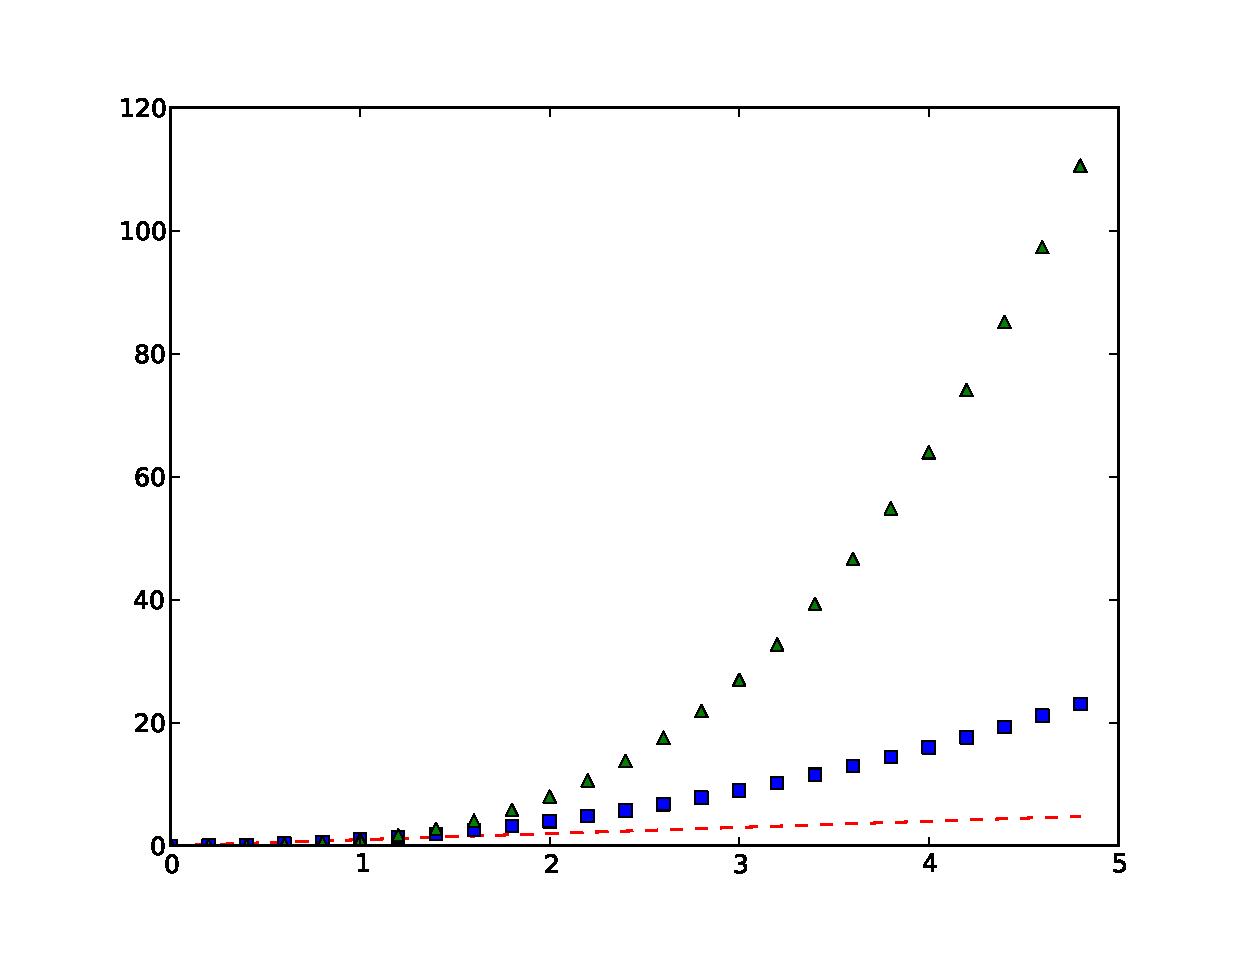
\includegraphics[scale=0.475]{Imagenes/plotEjercicio3.eps}
\end{figure}
\end{frame}
\begin{frame}[fragile]
\frametitle{Ejercicio de graficación 4}
Trabajando con múltiples gráficas. \pause En ocasiones vamos a necesitar mostrar dos (o más gráficas) para un mismo problema: por ejemplo graficar el cambio de distancia y la velocidad de un móvil, ambas variables en gráficas separadas.
\\
\bigskip
\pause
Esta tarea se resuelve de manera sencilla como veremos en el siguiente ejemplo.
\end{frame}
\begin{frame}[allowframebreaks, fragile]
\frametitle{Ejercicio de graficación 4}
\begin{lstlisting}
import numpy as np
import matplotlib.pyplot as plt

def f(t):
    return np.exp(-t) * np.cos(2*np.pi*t)

t1 = np.arange(0.0, 5.0, 0.1)
t2 = np.arange(0.0, 5.0, 0.02)

plt.figure(1)
plt.subplot(211)
plt.plot(t1, f(t1), 'bo', t2, f(t2), 'k')

plt.subplot(212)
plt.plot(t2, np.cos(2 * np.pi * t2), 'r--')
\end{lstlisting}
\end{frame}
\begin{frame}[fragile]
\frametitle{Subplots obtenidas}
\begin{figure}
	\centering
	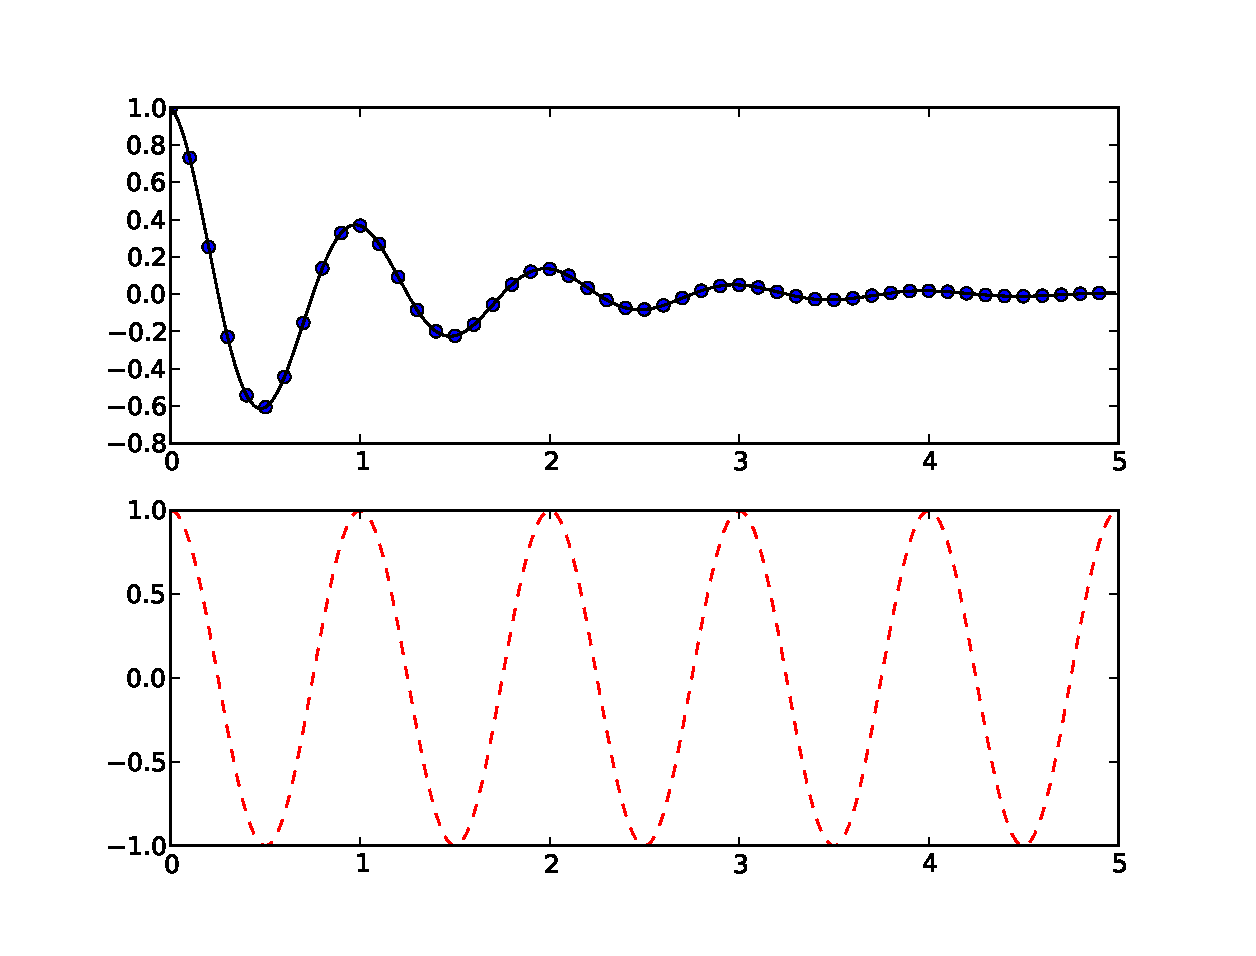
\includegraphics[scale=0.475]{Imagenes/plotEjercicio4.eps}
\end{figure}
\end{frame}
\begin{frame}
\frametitle{Las instrucciones para los subplots}
El comando \funcionazul{figure()} aquí es opcional, ya \funcionazul{figure(1)} se crea de forma predeterminada, \pause así mismo \funcionazul{subplot(111)} se crea de forma predeterminada si no se especifica manualmente un eje.
\end{frame}
\begin{frame}
\frametitle{Las instrucciones para los subplots}
El comando \funcionazul{subplot()} especifica \texttt{numrows, numcols, fignum} donde \texttt{fignum} varía en rango de 1 a \texttt{numrows * numcols}.
\\
\bigskip
\pause
Las comas en el comando \funcionazul{subplot()} son opcionales si \texttt{numrows * numcols} $<10$. Por tanto \texttt{subplot(211)} es idéntica a la \texttt{subplot(2,1,1)}.
\end{frame}
\begin{frame}
\frametitle{Más recursos para graficar con \python}
Lo que hemos visto es una revisión muy básica y general de cómo generar una gráfica con \python, hay todavía una enorme cantidad de información sobre \funcionazul{matplotlib}, encontrarás en la página oficial de la librería, bastante documentación, ejemplos y elementos para extender completamente esta herramienta.
\end{frame}
\begin{frame}
\frametitle{Más recursos para graficar con \python}
Se les proporcionará una guía breve de graficación, con la intención de que revisen casos prácticos aplicados a la física. Para cada gráfica que usemos más adelante en el curso, tendrán oportunidad de agregar más elementos que ustedes consideren.
\end{frame}
\end{document}